\section{Typisierung}
\begin{center}
	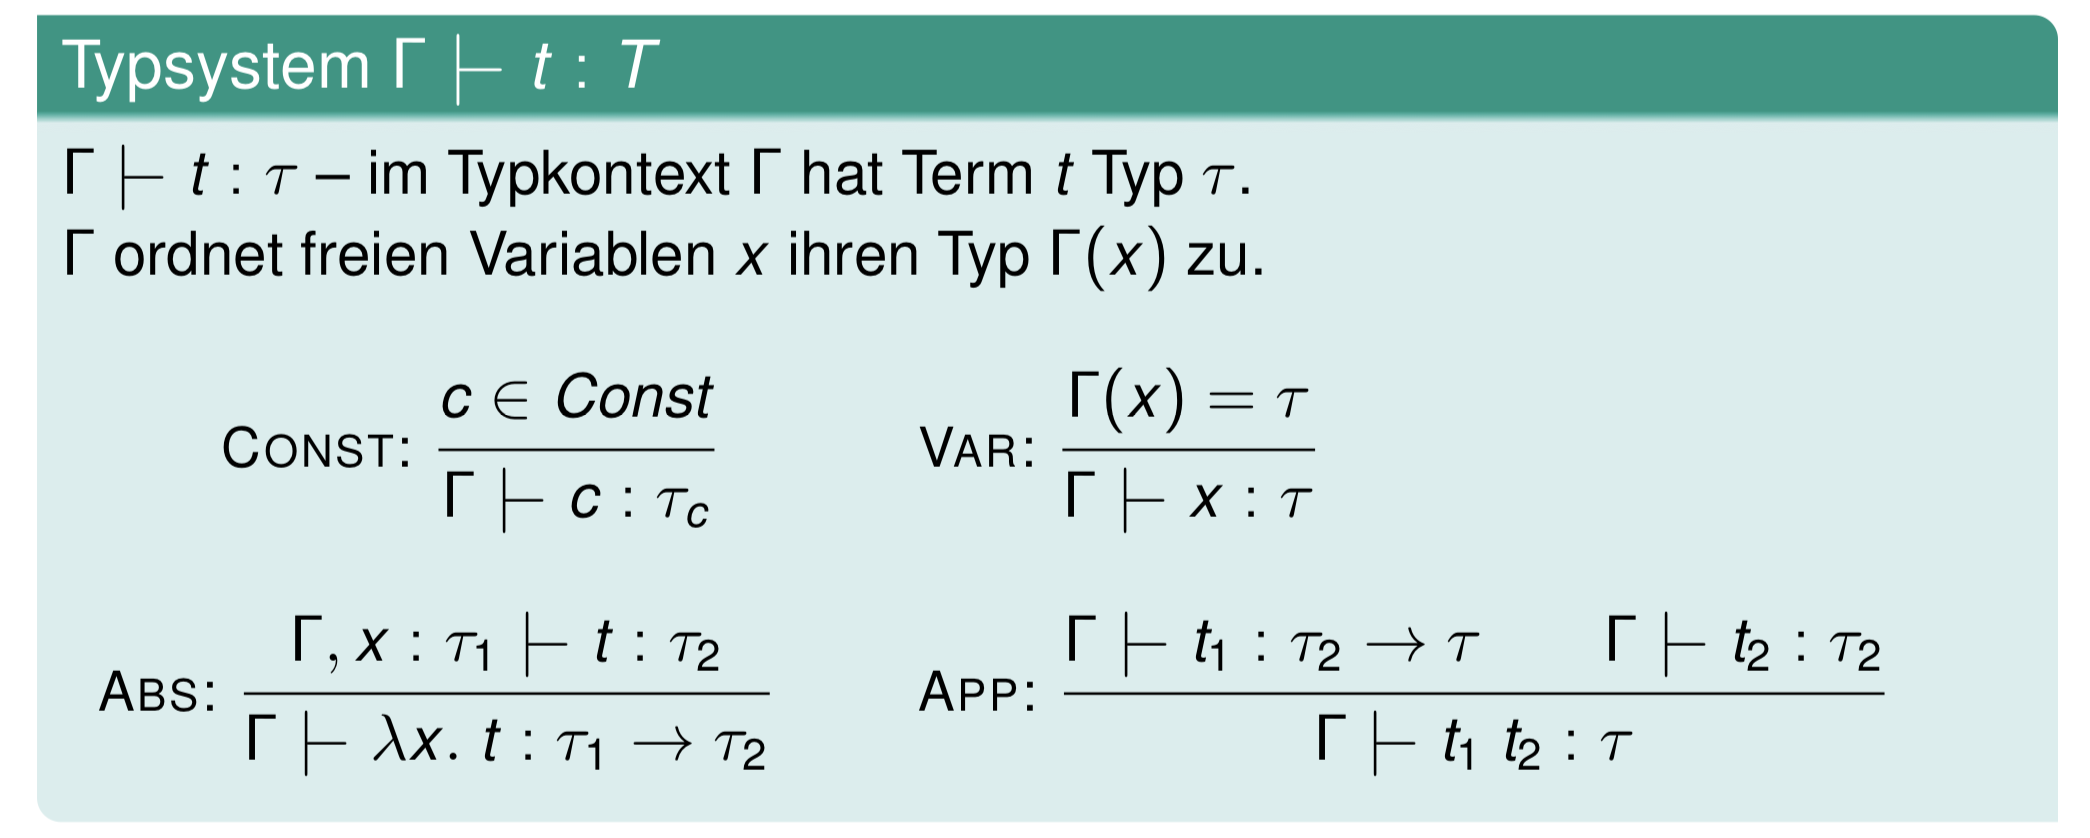
\includegraphics[width=\columnwidth]{images/types.png}	
\end{center}
\begin{center}
		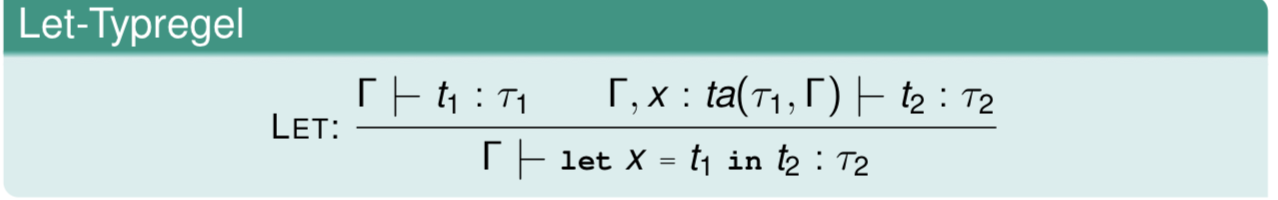
\includegraphics[width=\columnwidth]{images/let.png}
\end{center}
Beispiel:\\
\begin{center}
	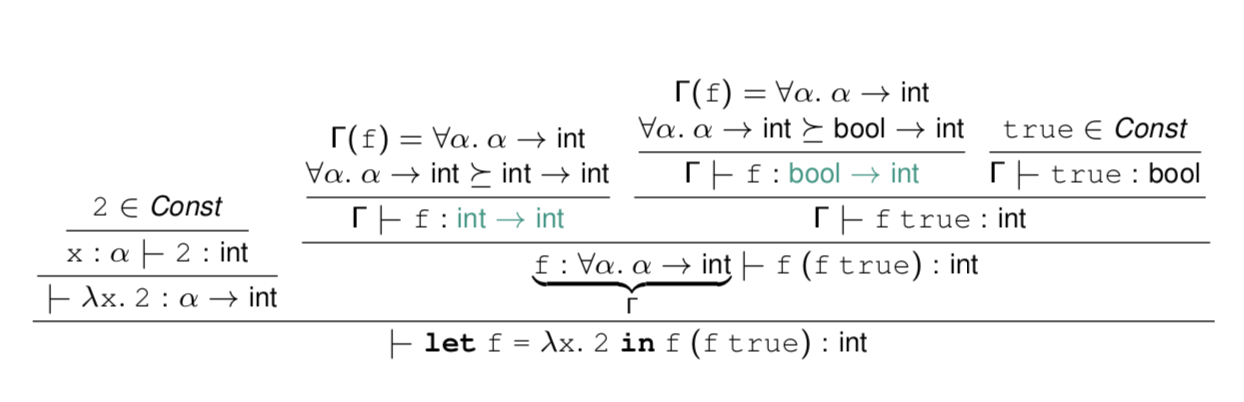
\includegraphics[width=\columnwidth]{images/let_ex.png}
\end{center}
\subsection{Constraint basierte Typisierung}

\begin{enumerate}
	\item Erstelle Herleitungsbaum. Verwende immer frische Typvariablen $\alpha_i$. Beginnend unten mit $\alpha_1$
	\item Stelle Constraints $C$ für die $\alpha_i$ auf (siehe \ref{typ:con:crea})
	\item Bestimme $\sigma_{mgu}$ der die Gleichungen löst
	\item Typ: $\sigma_{mgu}(\alpha_1)$
\end{enumerate}

\subsubsection{Constrainterstellung}
\label{typ:con:crea}
$$APP \medspace\frac{\Gamma \vdash t_1 : \alpha_2 \medspace\medspace\medspace \Gamma \vdash t_2 : \alpha_3}{\Gamma \vdash t_1 \medspace t_2 : \alpha_1} \rightsquigarrow C = C_0 \cup \{\alpha_2 = \alpha_3 \rightarrow \alpha_1\}$$

$$ABS \medspace\frac{\Gamma, x : \alpha_2 \vdash t : \alpha_3}{\Gamma \vdash \lambda x.t:\alpha_1} \rightsquigarrow C = C_0 \cup \{\alpha_1 = \alpha_2 \rightarrow \alpha_3\}$$

$$VAR \medspace\frac{(x: \alpha_1)(x) = \alpha_2}{\Gamma \vdash x : \alpha_2} \rightsquigarrow C = C_0 \cup \{\alpha_1 = \alpha_2\}$$

$$Const \medspace\frac{c \in Const}{\Gamma \vdash x : \alpha_1} \rightsquigarrow C = C_0 \cup \{\alpha_1 = \alpha_c\}$$

\subsubsection{Let}
Betrachte:
$$\frac{\Gamma \vdash t_1: \alpha_2 \medspace \Gamma' \vdash t_2: \alpha_3}{\Gamma \vdash \textbf{let } x = t_1 \textbf{ in } t_2 : \alpha_1}$$

\begin{enumerate}
	\item Setze $C_0 \coloneqq \{ \alpha_1 = \alpha_3 \}$
	\item Bestimme $C_{let}$ (linker Teilbaum) und $\sigma_{C_{let}}$
	\item Sei $\Gamma_r$ Typannahme rechter Teilbaum, dann ist $\Gamma_r = \Gamma, x: \forall \alpha. ...$
	\item Bestimme $C_{let}' = \{\alpha_i = \sigma_{let}(\alpha_i)\}$
	\item Bestimme constraints rechter Teilbaum $C_r$
	\item Bestimme $\sigma_{(C_0 \cup C_r \cup C_{let}')}$
\end{enumerate}